% \section{Architecture}
\label{sec:arch}
Modern speech recognition and speech translation systems are predominantly built on the encoder-decoder paradigm. In this framework, the encoder extracts high-level representations from the raw speech signal, conditioning the decoder to generate text in the target language. The most powerful recent systems employ pure Transformer-based architectures, often trained at a massive speech scale data. For instance, Whisper \cite{radford2023whisper} demonstrated that training a Transformer encoder-decoder on hundreds of thousands of hours of weakly supervised multilingual data yields state-of-the-art performance on both Automatic Speech Recognition (ASR) and Speech Translation (ST) tasks. Similarly, SeamlessM4T \cite{barrault2023seamlessm4t} extended this approach to create a unified multilingual framework for speech and text translation, underscoring the scalability of Transformer-based designs. Earlier models, such as the Speech-Transformer \cite{dong2018speech}, were instrumental in establishing the viability of attention-based encoder-decoder architectures for speech processing.

In contrast to general-purpose Transformers, several architectures have been tailored specifically for speech. The Conformer \cite{gulati2020conformer} augments the Transformer with convolutional modules, enabling it to capture both fine-grained local acoustic patterns and long-range global dependencies. Its optimized variant, the FastConformer \cite{rekesh2023fastconformer}, further enhances efficiency through aggressive subsampling and the use of depthwise separable convolutions. Such encoders are often paired with online decoders like the RNN-Transducer (RNN-T) \cite{jain2019rnntransducer}, Token and Duration Transducer (TDT)\cite{xu2023efficient} or Connectionist Temporal Classification (CTC) \cite{graves2006connectionist}, which are widely adopted for streaming ASR due to their low-latency characteristics.

For speech translation, however, autoregressive Transformer-based decoders remain dominant, as they excel at modeling cross-lingual dependencies and generating fluent text. Recently, a prominent strategy has been to integrate pre-trained Large Language Models (LLMs) as decoders. This approach leverages the vast linguistic knowledge captured during text-only pre-training and scales effectively across modalities. For example, models like SALM\cite{chen2024salm}\footnote{\url{https://huggingface.co/nvidia/canary-qwen-2.5b}}, BESTOW \cite{chen2024bestow} and SpeechGPT \cite{zhang2023speechgpt} adapt speech encoders to interface with powerful LLMs. One example of such integration is Phi-4-Multimodal \cite{abouelenin2025phi4multimodal}. In this architecture, inputs from multiple modalities—including speech—are processed by modality-specific encoders (e.g., a Conformer for speech). The resulting features are projected into a common embedding space via lightweight adapters and then decoded by a shared LLM backbone (Phi-4-Mini) equipped with LoRA adapters for speech-to-text tasks. This design circumvents traditional decoder retraining by adapting the LLM with LoRA, efficiently enabling language generation conditioned on speech inputs.

 Notable approach from above models is the Speech-Augmented Language Model (SALM) \cite{chen2023salm}, which utilizes a frozen pre-trained text LLM and augments it with a speech encoder, a modality adapter, and LoRA layers. This creates a unified architecture for both ASR and ST. Trained with in-context speech instruction tuning, SALM matches the performance of specialized Conformer models while also demonstrating zero-shot adaptation and keyword boosting capabilities. Such designs not only improve translation quality but also align speech models more closely with the architectural principles of today's leading text-based systems.

\subsection{Encoder}
In any encoder-decoder architecture for speech, the encoder is a critical component. It is typically responsible for the majority of the model's memory consumption. The full self-attention mechanism in encoder layers often becomes the primary bottleneck during pre-training and inference, especially with long audio sequences. Consequently, the encoder's design plays a central role in determining both the scalability and efficiency of the entire system. Even minor architectural modifications or scaling decisions can yield substantial performance gains. In this work, we focus on the encoder and experiment with two distinct architectures: the FastConformer \cite{rekesh2023fast} and the normalized GPT (nGPT) \cite{loshchilov2024ngpt}.

\subsubsection{FastConformer}
The FastConformer is an evolution of the Conformer encoder, explicitly optimized for computational efficiency in speech tasks. Its primary improvements over the original Conformer include:

\begin{itemize}
    \item \textbf{Aggressive Subsampling (8x):} Input features are downsampled by a factor of 8 at the input stage using convolutional blocks. This significantly shortens the sequence length, reducing computational cost while preserving accuracy.
    \item \textbf{Depthwise Separable Convolutions:} Standard convolutions in both the subsampling layers and the Conformer blocks are replaced with depthwise separable convolutions, which reduces the number of operations while maintaining strong performance.
    \item \textbf{Lightweight Convolutional Modules:} The convolutional kernel size is reduced (e.g., from 31 to 9) and channel dimensions are scaled down, further streamlining the encoder without degrading recognition quality.
\end{itemize}

These optimizations yield a model that is significantly faster (2–3× inference speedup) and more memory-efficient, while achieving accuracy comparable to or better than the original Conformer.

\vspace{0.3em} % space before figure
\begin{figure}[htbp]
    \centering
    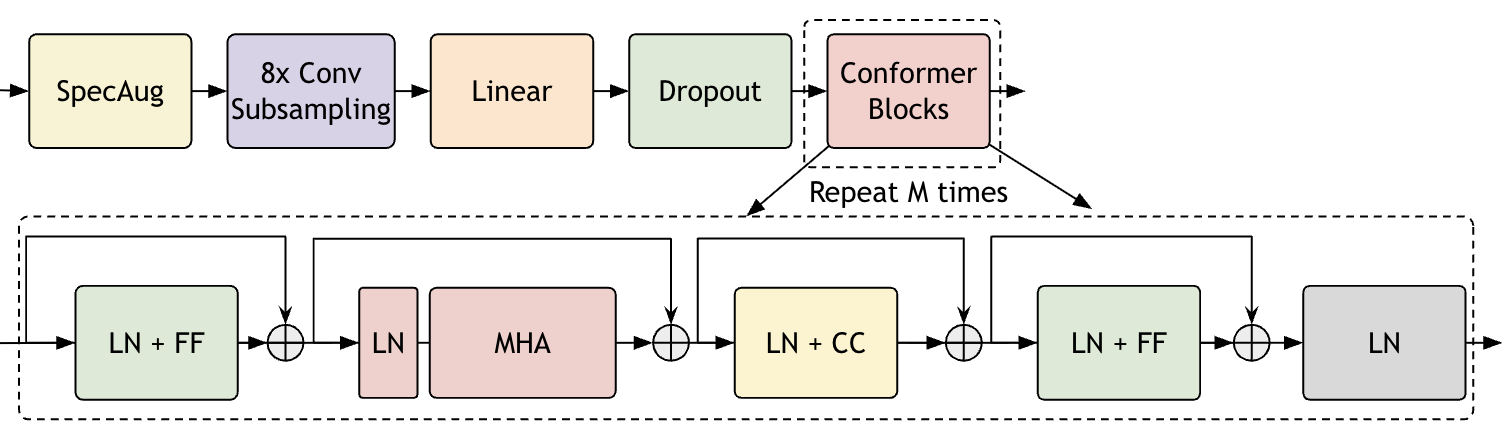
\includegraphics[width=0.8\textwidth]{images/fastconformer.png}
    \caption{Overview of the \textbf{FastConformer} architecture. The input features are first subsampled to a resolution of 80\,ms, followed by a linear projection and dropout for dimensionality reduction and regularization. The core of the model consists of a stack of repeated Conformer blocks, each containing four main components: Layer Normalization (LN), a Feed-Forward (FF) module, a Multi-Head Attention (MHA) mechanism, and a Convolutional Module (CC).}
    \label{fig:fastconformer}
\end{figure}


\subsubsection{nGPT}
While the FastConformer optimizes a speech-specific architecture, a different line of research has focused on fundamentally rethinking the Transformer itself. Normalized GPT (nGPT) model \cite{loshchilov2024ngpt}  introduces a hyperspherical normalization scheme that constrains all embeddings to a unit hypersphere. This design stabilizes training, improves generalization, and accelerates convergence, enabling the model to reach target validation metrics in fewer steps than standard Transformers.

Building on these ideas, we adapt nGPT into a full encoder-decoder architecture for speech. To the best of our knowledge, this is the first work to explore the nGPT architecture for speech processing tasks. As an initial step, we developed and evaluated an nGPT-based encoder, allowing us to isolate and study its effectiveness in the acoustic domain. For the decoder, we retained a conventional Transformer architecture to ensure that any observed improvements could be directly attributed to the novel encoder design.

Our implementation of the \texttt{NGPTEncoder} begins with a Linear subsampling front-end to reduce the temporal resolution of the input spectrogram. The encoder is then constructed as a stack of nGPT layers, with the following key components:

\begin{itemize}
    \item \textbf{Multi-head Attention with Rotary Embeddings.} The attention layers use Rotary Positional Embeddings (RoPE) for long-sequence generalization and standard scaled dot-product attention.
    \item \textbf{Feed-forward Network.} Each layer uses a gated two-stage feed-forward module with a SiLU activation.
    \item \textbf{Hyperspherical Normalization.} All embeddings and intermediate activations are constrained to lie on a unit hypersphere. Query, key, and projection weights are explicitly normalized, with learnable scaling factors ($\alpha, \sigma$) regulating the residual contributions from the attention and feed-forward modules.
    \item \textbf{Residual Connections.} Residual paths can be interpreted as a first-order optimization step, where each layer refines the representation by adding an incremental update to the current state.
\end{itemize}

\vspace{0.3em} % space before figure
\begin{figure}[htbp]
    \centering
    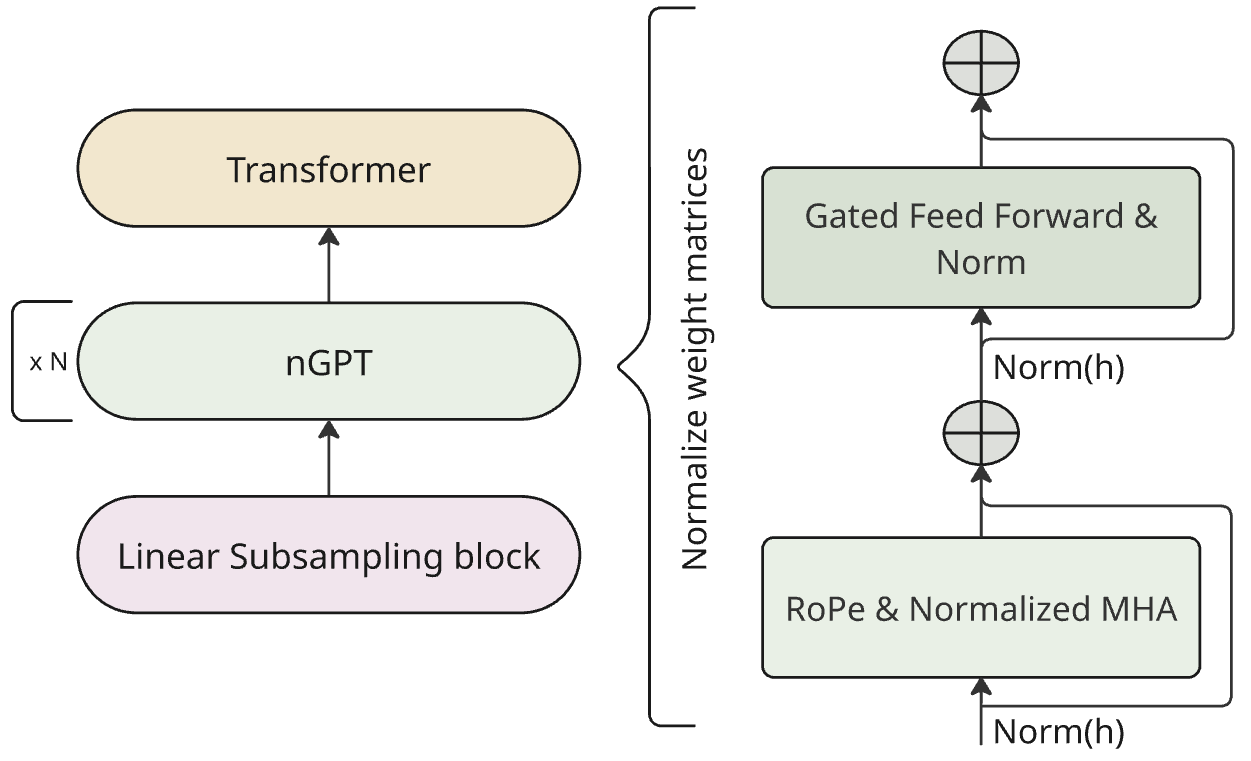
\includegraphics[width=0.5\textwidth]{images/ngpt.png}
    \caption{Overview of the nGPT architecture. The input features are first processed by a linear subsampling block. This is followed by a stack of repeated nGPT layers and a Transformer decoder. Each nGPT layer adopts a Transformer-style design with Rotary Position Embeddings (RoPE), multi-head attention, and gated feed-forward modules. Normalization is applied across the embedding dimension, and both activations and weight matrices are normalized, with weight normalization additionally enforced after each optimizer update.}
    \label{fig:ngpt_architecture}
\end{figure}


\subsubsection{Positional Encodings}
Our initial nGPT implementation adopted Rotary Positional Encodings (RoPE) \cite{su2021roformer} as the baseline. RoPE injects position information by applying a rotation to the query and key vectors, a design known to generalize well in long-context settings. While functional, our experiments with RoPE revealed performance degradation in very long-context ASR and ST scenarios.

To address this limitation, we explored Attention with Linear Biases (ALiBi) \cite{press2022alibi}. ALiBi was originally designed for autoregressive language models, where it adds a static, position-dependent bias to the attention scores, penalizing attention to distant tokens. Since our encoder processes the full context (i.e., it is bidirectional), we modified the original ALiBi formulation to use a symmetric bias matrix, ensuring that both left and right contexts are treated equally. This adaptation allowed us to integrate ALiBi into our nGPT encoder as an alternative positional encoding scheme. This represents the first exploration of ALiBi positional embeddings for speech recognition and translation tasks.

\vspace{0.3em} % space before figure
\begin{figure}[htbp]
    \centering
    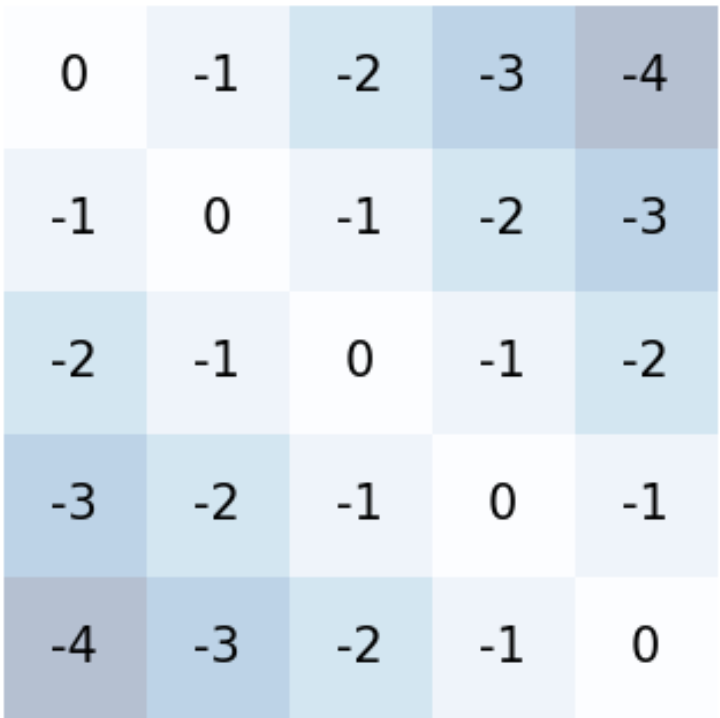
\includegraphics[width=0.2\textwidth]{images/alibi.png}
    \caption{Symmetric ALiBi bias matrix used in the nGPT encoder. Unlike the original causal ALiBi, which penalizes only future positions, this non-causal variant applies equal bias to tokens before and after the current position, ensuring balanced treatment of left and right context.}

    \label{fig:alibi_matrix}
\end{figure}